\documentclass[]{article}
\usepackage{geometry}
\geometry{a4paper, margin=1in}
\usepackage{amssymb}
\usepackage{multirow}                                                      % you want to use the \thanks command
%\usepackage{multicolumn}
\usepackage{amsmath}
\usepackage{amsfonts}
%\usepackage{math}
\usepackage{adjustbox}
%\usepackage{graphics}
\usepackage{subfigure}
\setcounter{tocdepth}{3}
\usepackage{graphicx}
\usepackage{xcolor}
%\usepackage{url,hyperref,lineno,microtype}
%\usepackage[onehalfspacing]{setspace}
%\usepackage{amssymb}
%\usepackage{subfigure}
%\usepackage{bm}
%\usepackage{multirow}
\usepackage{amsbsy}
%\usepackage{color}
%\usepackage{cite}
%\setcounter{tocdepth}{3}
%\usepackage{graphicx}

\newcommand{\tr}{\operatorname{tr}}
\newcommand{\gD}[2]{\mathcal{N}\left(#1,#2\right)}
\newcommand{\dWj}{\partial\projMat}
\newcommand{\kernel}[2]{k\left(#1,#2\right)}
\newcommand{\kernelww}[2]{k\left(\mathbf{w}_{#1}^d,\mathbf{w}_{#2}^d\right)}
\newcommand{\kernelwx}[1]{k\left(\mathbf{w}_{#1}^d,\indobj\right)}
\newcommand{\catD}[2]{\mathcal{G}\left(#1,#2\right)}
\newcommand{\Z}{\boldsymbol{\mathrm{Z}}}
\newcommand{\C}{\boldsymbol{\Lambda}_j}
\newcommand{\Cin}{\mathbf{C}_j}
\newcommand{\muJ}{\boldsymbol{\mu}_j}
\newcommand{\gammaA}{\Gamma\left(a\right)}
\newcommand{\eye}{\mathbf{I}}
\newcommand{\Scluster}{\mathbf{S}}
\newcommand{\W}{\boldsymbol{\mathcal{W}}}

\newcommand{\WIn}{\mathbf{W}}
\newcommand{\setWv}{\mathbf{W}^{v}}
\newcommand{\setYv}{\mathbf{Y}^{v}}
\newcommand{\setY}{\mathbf{Y}}
\newcommand{\setXv}{\mathbf{X}^{v}}
\newcommand{\setZv}{\mathbf{Z}^{v}}
\newcommand{\setFv}{\mathbf{F}^{v}}
\newcommand{\setKv}{\mathbf{K}^{v}}
\newcommand{\setX}{\mathbf{X}}
\newcommand{\setObj}{\mathbf{X}_d}
\newcommand{\indobj}{\mathbf{x}_{dn}}
\newcommand{\projMat}{\boldsymbol{\mathcal{W}}_d}

\newcommand{\hParams}{\boldsymbol{\theta}}
\newcommand{\hParamsv}{\boldsymbol{\theta}^{v}}

\newcommand{\obspv}{\mathbf{x}_{nv}}
\newcommand{\projMatI}{\mathbf{W}_d}
\newcommand{\dWjIn}{\partial\projMatI}
\newcommand{\lvecI}{\mathbf{z}_j}
\newcommand{\lvecsI}{\mathbf{z}_{s_{dn}}}
\newcommand{\lvec}{\boldsymbol{\zeta}_j}
\newcommand{\lvecs}{\boldsymbol{\zeta}_{s_{dn}}}
\newcommand{\mixwe}{{\theta}_j}
\newcommand{\mapphi}{\phi\left(x\right)}
\newcommand{\mapphit}{\phi\left(x'\right)}
\newcommand{\comment}[2]{{\color{blue}#1} {\color{red}#2}}
\newcommand{\phixnd}{\boldsymbol{\phi}\left(\indobj\right)}
\newcommand{\phiwld}[1]{\boldsymbol{\varphi}\left(\mathbf{w}_{#1}^d\right)}
\newcommand{\phiwldI}[2]{\varphi_{#2}\left(\mathbf{w}_{#1}^d\right)}
\newcommand{\wH}{\boldsymbol{\omega}_{j}^d}
\newcommand{\wHj}[1]{\boldsymbol{\omega}_{#1}^d}
\newcommand{\wIj}[1]{\mathbf{w}_{#1}^d}
\newcommand{\muJFa}{\sum_{d=1}^{D}\mathbf{\hat{k}}_d }
\newcommand{\kawx}{\mathbf{\hat{k}}_d }
\newcommand{\Kaww}{\mathbf{\hat{K}}_d }
\newcommand{\dWd}{\partial \boldsymbol{\Theta}}
\newcommand{\likel}{\log p\left(\boldsymbol{\Phi},\mathbf{S}|\W,a,b,r,\gamma\right)}
\newcommand{\GP}[2]{\mathcal{GP}\left(#1,#2\right)}


%%%%%%% iWMM params
\newcommand{\lambdac}{\lambda_c}
\newcommand{\muC}{\boldsymbol{\mu}_c}
\newcommand{\RC}{\mathbf{R}_c}


%\everymath{\displaystyle}
%\everymath{\scriptstyle}
%opening
\title{Multi-view Warped Mixtures for Shape Correspondence Analysis}
\author{Hern\'an F. Garc\'ia and Mauricio A. \'Alvarez}

\begin{document}

\maketitle

\begin{abstract}
Probabilistic approach for the correspondence problem based on the Single View WMM\cite{IwaDuvGha2012warped}.
\end{abstract}

\section{Multiview Warped Mixture Models}

We can use the single view problem of the warped mixture model from \cite{IwaDuvGha2012warped} in which they warp a latent mixture of Gaussians into nonparametric cluster shapes. The low-dimensional latent mixture model summarizes the properties of the high-dimensional density manifolds describing the data.

Our idea is to introduce a model which warps a multiview latent mixture of Gaussians (possibly MRD) to produce nonparametric cluster shapes. \footnote{The possibly low-dimensional latent mixture model allows us to summarize the properties of the high-dimensional clusters
(or density manifolds) describing the data. The number of manifolds, as well as the shape and dimension of each manifold is automatically inferred.}


%\begin{figure}[h!]
%	\centering
%	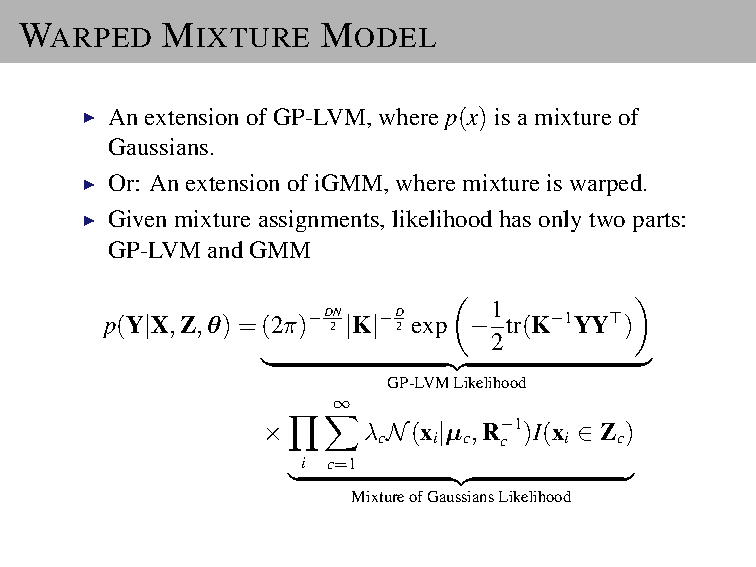
\includegraphics[width=.9\linewidth]{img/iwmm_talk_Model}
%	\caption{WMM from \cite{IwaDuvGha2012warped}}
%\end{figure}

\subsection{The model}

Let as define a multi-view data set as $\mathcal{Y}=\left\{\mathbf{Y}^{v}\right\}_{v=1}^{V}$, where each view is defined as $\mathbf{Y}^{v}\in \mathbb{R}^{N_v\times D_v}$. This leads to the likelihood Given mixture assignments, likelihood has only two parts:
GP-LVM and GMM

\begin{align}
p\left(\mathbf{Y}^{\mathcal{V}}|\mathbf{X},\mathbf{Z},\boldsymbol{\theta}\right) = \prod_{v=1}^{V}p(\mathbf{Y}^v|\mathbf{X},\boldsymbol{\theta})\times \prod_{i}\sum_{c=1}^{\infty} \lambda_c\gD{\mathbf{x}_i|\boldsymbol{\mu}_c}{\mathbf{R}_c^{-1}} ,\quad \mathbf{x}_i \in \mathbf{Z}_c
\end{align}


Based on the iWMM (see \cite{IwaDuvGha2012warped}) our generative model generates multiple observations $\mathbf{Y}^{\mathcal{V}}$ according to the following generative process:

\begin{enumerate}
	\item Draw mixture weights $\boldsymbol{\lambda}\sim \operatorname{GEM}(\eta)$
	\item For each cluster $c = 1, \cdots,\infty $
	\begin{enumerate}
		\item Draw precision $\mathbf{R}_c \sim \mathcal{W}(\mathbf{S}^{-1},v)$
		\item Draw mean $\boldsymbol{\mu}_c \sim \mathcal{N}(\mathbf{u},(r\mathbf{R}_c)^{-1})$
	\end{enumerate}
	
	\item For each view $v = 1, \cdots,\mathcal{V} $
	\begin{enumerate}
		\item For each observation $n = 1,\cdots,N_v$
	\begin{enumerate}
		\item Draw latent assignment $z_{nv} \sim \operatorname{Mult}(\boldsymbol{\lambda})$
		\item Draw latent coordinates $\mathbf{x}_{nv} \sim \mathcal{N}(\boldsymbol{\mu}_{z_{nv}},\mathbf{R}_{z_{nv}}^{-1})$
	\end{enumerate}
	\end{enumerate}

	\item For each view $v = 1, \cdots,\mathcal{V} $
	\begin{enumerate}
		\item For each observed dimension $d = 1,\cdots,D_v$
		\begin{enumerate}
			\item Draw function $\mathbf{f}_{d}^{v} \sim \mathcal{GP}(\mathbf{0},\mathbf{K}^{v})$
		\end{enumerate}
	\end{enumerate}

	\item For each view $v = 1, \cdots,\mathcal{V} $
			
			
	\begin{enumerate}
		
		\item For each observed dimension $d = 1,\cdots,D_v$

		\begin{enumerate}
					\item Draw projection variable ${w}_{d}^v\sim \gD{0}{\rho_d^v}$
			\item For each observation $n = 1,\cdots,N_v$
			\begin{enumerate}
				\item Draw feature $y_{nd}^{v}\sim \gD{\textcolor{red}{{w}_{d}^v}f_d^{v}(\mathbf{x}_{nv})}{\beta^{-1}}$
			\end{enumerate}
		\end{enumerate}
	\end{enumerate}
\end{enumerate}

We define the dimensionalities of our variables as:

\begin{itemize}
	\item 	$K$: real number of clusters
	\item $Q$:  dimensionality of the Latent Space
	\item $D_v$: dimensionality of the input data in the $v$-th view 
	\item $\boldsymbol{\lambda} \in \mathbb{R}^{K\times 1}$ 
	\item $\mathbf{R}_c \in \mathbb{R}^{Q\times Q}$
	\item $\boldsymbol{\mu}_c \in \mathbb{R}^{Q\times 1}$
\end{itemize}


%\textbf{Question:} Can we relate the outputs $y_{nd}$ through multi-output GPs?

\subsection{Latent Multi-view Warped Mixture Model}

Our model is set as a multi-view Gaussian Process Latent Variable model as \cite{Lawrence03}. First we assume 
that observations are generated by mapping the latent coordinates through a set of smooth functions, over
which Gaussian process priors are placed. Under the GPLVM, the probability of observations given the latent
coordinates, integrating out the mapping functions, is defined as

\begin{align}
p\left(\setY|\setX,\hParams\right) &= \prod_{v=1}^{V}p\left(\setYv|\setXv,\hParamsv\right) \\
   &= \prod_{v=1}^{V}\prod_{d=1}^{D_v}p\left(\mathbf{y}_d^v|\setXv,\hParamsv\right),
\end{align}


where $\mathbf{y}_d^v$ represents the $d$th column of $\setYv$ and

\begin{align}
p\left(\mathbf{y}_d^v|\setXv,\hParamsv\right) = \gD{\mathbf{y}_d^v|\mathbf{0}}{\beta^{-1}\eye + w_d^2\setKv}.
\end{align}

Our multi-view iWMM assumes that the latent coordinates (per View) are generated from a Dirichlet process mixture model. In particular, we use the following infinite Gaussian mixture model,

\begin{align}
p(\mathbf{x}^{v}|\lambdac,\muC,\RC) = \sum_{c=1}^{\infty}\lambdac \gD{\mathbf{x}^{v}|\muC}{\RC^{-1}},
\end{align}

where $\lambdac$, $\muC$ and $\RC$ are the mixture weight, mean, and
precision matrix of the $c$th mixture component.

As in the iWMM \cite{IwaDuvGha2012warped}, we
place Gaussian-Wishart priors on the Gaussian parameters $\left\{\muC,\RC\right\}$.

\begin{align}
p\left(\muC,\RC\right) = \gD{\muC|\mathbf{u}}{(r\RC)^{-1}}\mathcal{W}\left(\RC|\mathbf{S}^{-1},\nu\right)
\end{align}

where $\mathbf{u}$ is the mean of $\muC$, $r$ is the relative precision of $\muC$, $\mathbf{S}^{-1}$ is the scale matrix for $\RC$, and $\nu$ is the number of degrees of freedom for $\RC$.


By using conjugate Gaussian-Wishart priors for the parameters
of the Gaussian mixture components, we can analytically
integrate out those parameters, given the assignments
of points to components. Let $z_n^{v}$ be the latent assignment
of the $n$th object in the $v$th view. The probability of latent coordinates $\mathbf{X}$ given latent assignments $\setZv = \left(z_1,\dots,z_{N_v}\right)$ is obtained by integrating out the Gaussian parameters $\left\{\muC,\RC\right\}$ as follows:


\begin{align}
p\left(\setX|\Z,\Scluster,\nu,r\right) = \prod_{c=1}^{\infty} \pi^{-\frac{\sum_v N_{vc}Q}{2}}\frac{r^{Q/2}|\Scluster|^{\nu/2}}{r_c^{Q/2}|\Scluster_c|^{\nu_c/2}}\prod_{q=1}^{Q}\frac{\Gamma\left(\frac{\nu_c + 1 -q}{2}\right)}{\Gamma\left(\frac{\nu + 1 -q}{2}\right)},
\end{align}

where $N_{vc}$ is the number of objects in the $v$th view assigned to the $c$th cluster, $\Gamma\left(\cdot\right)$ is the Gamma function and

\begin{align*}
r_c &= r + \sum_v N_{vc},\quad \nu_c = \nu + \sum_v N_{vc},\\
\mathbf{u}_c & = \frac{r\mathbf{u}+\sum_{v=1}^{V}\sum_{n:z_{nv} = c}\mathbf{x}_{nv}}{r+\sum_v N_{vc}},\\
\Scluster_c &= \Scluster + \sum_{v=1}^{V}\sum_{n:z_{nv} = c} \mathbf{x}_{nv}\mathbf{x}_{nv}^\top + r \mathbf{u}\mathbf{u}^\top - r_c \mathbf{u}_c\mathbf{u}_c^\top,
\end{align*}

are the posterior Gaussian-Wishart parameters of the
$c$th component. As in \cite{IwaDuvGha2012warped}, we use a Dirichlet process with concentration parameter $\eta$ for infinite mixture modeling in the latent space.

The probability of $\Z$ is given as follows 

\begin{align}
p\left(\Z|\eta\right) = \prod_{v=1}^{V}\frac{\eta^C \prod_{c=1}^{C}\left(N_{vc}-1\right)!}{\eta\left(\eta+1\right)\cdots\left(\eta+ N_v -1\right)},
\end{align}

where $C$ is the number of components for which $N_{vc} >
0$. The joint distribution is given by

\begin{align}
p\left(\setY,\setX,\Z|\hParams,\nu,\mathbf{u},r\eta\right) = \prod_{v=1}^{V}p\left(\setYv|\setXv,\hParamsv\right)p\left(\setXv|\Z_v,\Scluster_v , \nu,\mathbf{u},r\right)p\left(\Z_v|\eta\right).
\end{align}


\subsection{Inference}

We infer the posterior distribution of the latent coordinates
$\setX = \left\{\setXv\right\}_v^{V}$ and cluster assignments $\setZv$ using Markov
chain Monte Carlo (MCMC). In particular, we alternate
collapsed Gibbs sampling of $\Z$, and hybrid Monte
Carlo sampling of $\setX$. Given $\setX$, we can efficiently sample
$\setZv$ using collapsed Gibbs sampling, integrating out
the mixture parameters. Given $\setZv$, we can calculate the
gradient of the unnormalized posterior distribution of
$\setX$, integrating over warping functions. This gradient
allows us to sample $\setX$ using hybrid Monte Carlo.

First, we explain collapsed Gibbs sampling for Z.
Given a sample of X, $p\left(\Z|\setX,\Scluster,v,\mathbf{u},r,\eta\right)$ does not depend
on Y. This lets resample cluster assignments,
integrating out the iGMM likelihood in close form.
Given the current state of all but one latent component
zn, a new value for zn is sampled from the following
probability:

\begin{align*}
p\left(\mathbf{z}_{nv} = c| \setX,\Z_{\setminus nv},\Scluster,v,\mathbf{u},r,\eta\right) \propto \left\{\begin{array}{cc}
N_{vc\setminus{nv}}\cdot p\left(\obspv|\setX_c, \Scluster,v,\mathbf{u},r\right) & \textrm{existing components}\\
\eta\cdot p\left(\obspv|\Scluster,v,\mathbf{u},r\right) & \textrm{a new cluster}
\end{array}\right.
\end{align*} 

where $\setX_c = \left\{\obspv|\mathbf{z}_{nv}=c\right\}$ is the set of latent coordinates
assigned to the $c^{th}$ component, and $\setminus{nv}$ represents
the value or set when excluding the $n$-th observation in the $v$-th view. We can analytically calculate $p\left(\obspv|\setX_c, \Scluster,v,\mathbf{u},r\right)$  as follows:

\begin{align*}
p\left(\obspv|\setX_c, \Scluster,v,\mathbf{u},r\right) = \pi^{-\frac{N_{vc\setminus n}Q}{2}}\frac{r^{Q/2}|\Scluster|^{\nu/2}}{r_c^{Q/2}|\Scluster_c|^{\nu_c/2}}\prod_{q=1}^{Q}\frac{\Gamma\left(\frac{\nu_c + 1 -q}{2}\right)}{\Gamma\left(\frac{\nu + 1 -q}{2}\right)}
\end{align*}


\section{Results}

\section{Clustering performance on real datasets}

\begin{table*}[ht!]
	\centering
	\caption{Average Rand index for evaluating clustering performance.}
	\label{tab:comparison1}
	\begin{tabular}{c c c c c c c}
		\cline{2-7}
		& \multicolumn{5}{c}{\textbf{Database}}\\
		\hline
		\textbf{Approach} &  	Wine & 2-curve & 3-semi & 2-circle & Pinwheel& Vowel\\
		\hline\hline
%		iGMM  & $0.72\pm0.06$ &&&&&\\
%		iWMM ($Q=2$) & $0.65\pm0.05$ &&&&&\\
%		iWMM ($Q=D$) & $0.77\pm0.03$ &&&&&\\
		\hline
		MV-WMM($Q=2$) & $0.68\pm0.03$  &$0.83\pm0.02$ &$0.83\pm0.01$&$0.88\pm0.02$&$0.87\pm0.02$ & $0.65\pm0.01$\\
		MV-WMM($Q=D$) & $0.85\pm 0.02$ &$0.83\pm0.02$&$0.83\pm0.01$&$0.88\pm0.02$&$0.87\pm0.02$&$0.73\pm0.02$\\
		\hline

	\end{tabular}
\end{table*}

%2-curve 3-semi 2-circle Pinwheel Iris Glass Wine Vowel
%iGMM 0:52 0:79 0:83 0:81 0:78 0:60 0:72 0:76
%iWMM(Q=2) 0:86 0:99 0:89 0:94 0:81 0:65 0:65 0:50
%iWMM(Q=D) 0:86 0:99 0:89 0:94 0:77 0:62 0:77 0:76
\begin{figure}[ht!]
	\centering
	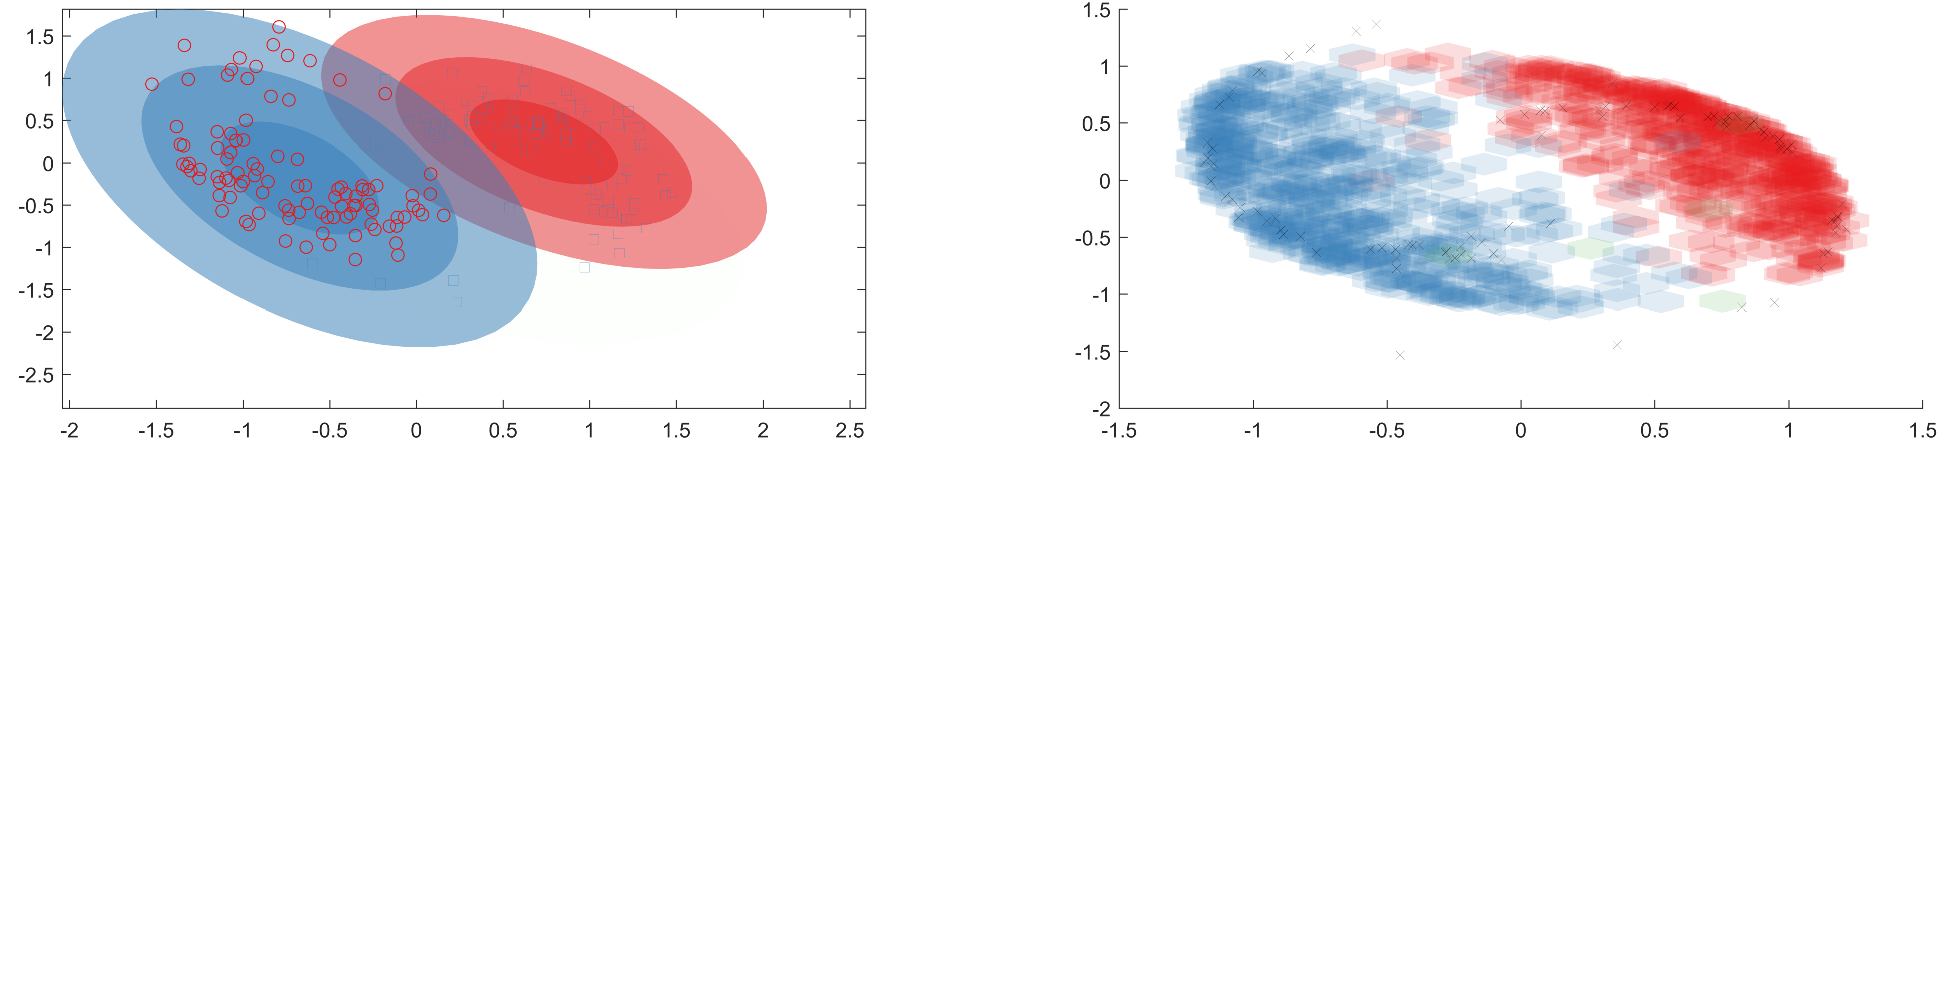
\includegraphics[width=0.9\linewidth]{img/mvwmmPW2arms100N}
	\caption{Experimental results for the Pinwheel dataset. Current mixture parameters, along with the latent positions (Top left). Original data and predicted assignments (Top right). }
\end{figure}


\subsection{Comparison with linear approaches}

First, we test the performance of our approaches (both NL-UCM and MV-WMM) regarding the adjusted Rand index (we report both average and standard deviation), to quantify the similarity between the inferred clusters \cite{Iwata16} and the true labels. For comparison, we use unsupervised clustering matching (UCM) \cite{Iwata16}, k-means (KM), and convex kernelized sorting (CKS) \cite{Djuric12}. Table \ref{tab:comparison} shows that our approaches outperforms the state-of-the-art methods for unsupervised clustering for the three databases. The results also show that by mapping the observed data through  random feature expansions, the model can handle real-world datasets with better performance than linear approaches as in the case of NL-UCM (i.e., $0.17$ for the MNIST dataset against $0.085$ obtained from the UCM method). 

\begin{table*}[ht!]
	\centering
	\caption{Adjusted Rand index of the proposed method against the state-of-the-art methods for unsupervised clustering.}
	\label{tab:comparison}
	\begin{tabular}{c c c c c c}
		\cline{2-6}
		& \multicolumn{4}{c}{\textbf{Approach}}\\
		\hline
		Database &  	UCM & KM & KM-CKS& \textbf{NL-UCM} & \textbf{MV-WMM}\\
		\hline\hline
		Iris & $0.383\pm0.189$ &  $0.224 \pm 0.0910$  &  $0.254 \pm 0.154$ &$\mathbf{0.546\pm 0.080}$ & $\mathbf{0.498\pm 0.001}$\\
		Glass & $0.160 \pm 0.020$ & $0.050 \pm 0.008$     &  $0.052 \pm 0.011$       & $\mathbf{0.378\pm 0.045}$ & $\mathbf{0.384\pm 0.003}$\\
		MNIST & $0.085 \pm 0.016$&      $0.030 \pm 0.007$   &  $0.037 \pm 0.008$  & $\mathbf{0.167\pm 0.013}$ & $\mathbf{0.133\pm 0.004}$\\
	\end{tabular}
\end{table*}

\subsection{Non-rigid 3D shape datasets}


\begin{figure}[ht!]
	\centering
	
		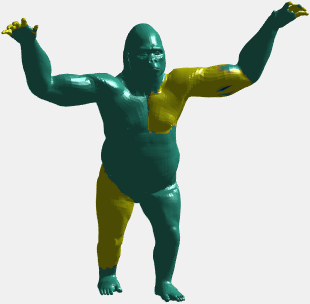
\includegraphics[width=0.43\linewidth]{img/gorillaAMVMMexp1}
			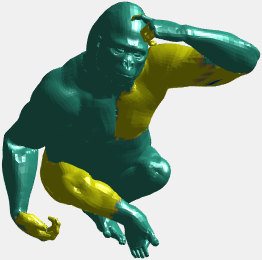
\includegraphics[width=0.4\linewidth]{img/gorillaAMVMMexp2}\\
	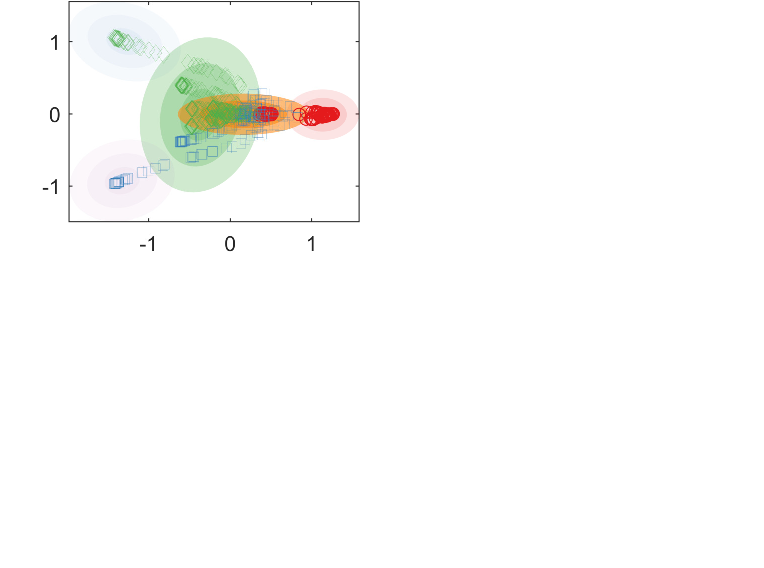
\includegraphics[width=0.45\linewidth]{img/GorillasMVWMM100Nexp2}
	\caption{Experimental results for the TOSCA dataset. Current mixture parameters, along with the latent positions for two shapes exhibiting different poses. Average Rand Index $0.6487$ }
\end{figure}

\begin{figure}[ht!]
	\centering
	
	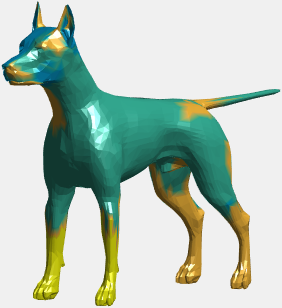
\includegraphics[width=0.43\linewidth]{img/dogMVWMM100Nexp2}
	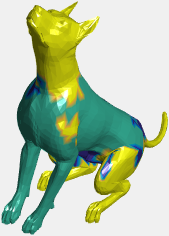
\includegraphics[width=0.34\linewidth]{img/dogMVWMM100Nexp2b}\\
%	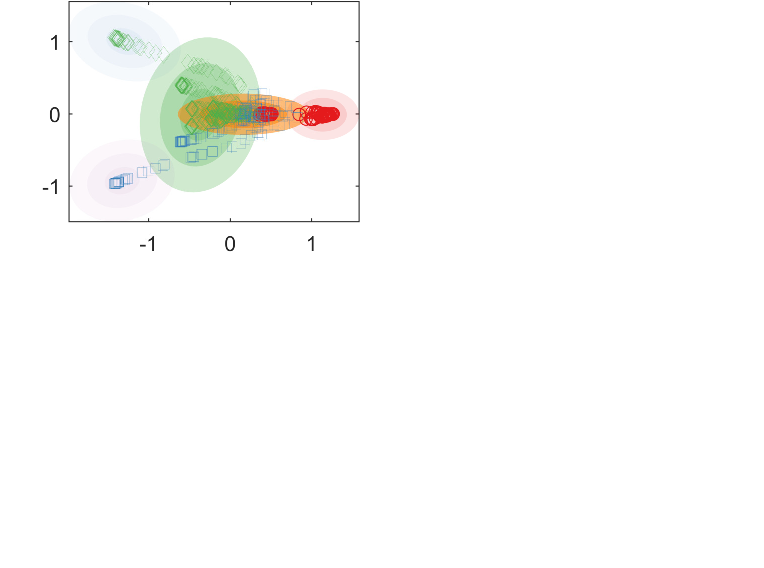
\includegraphics[width=0.45\linewidth]{img/GorillasMVWMM100Nexp2}
	\caption{Experimental results for the TOSCA dataset. Current mixture parameters, along with the latent positions for two shapes exhibiting different poses. Average Rand Index $0.5894$ }
\end{figure}

\begin{figure}[ht!]
	\centering
	
	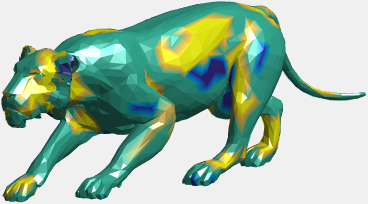
\includegraphics[width=0.43\linewidth]{img/lionlessMVMMexp1}
	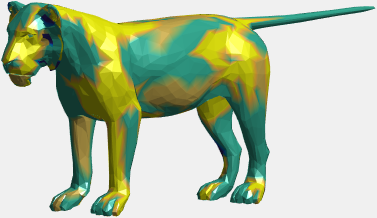
\includegraphics[width=0.41\linewidth]{img/lionlessMVMMexp2}\\
	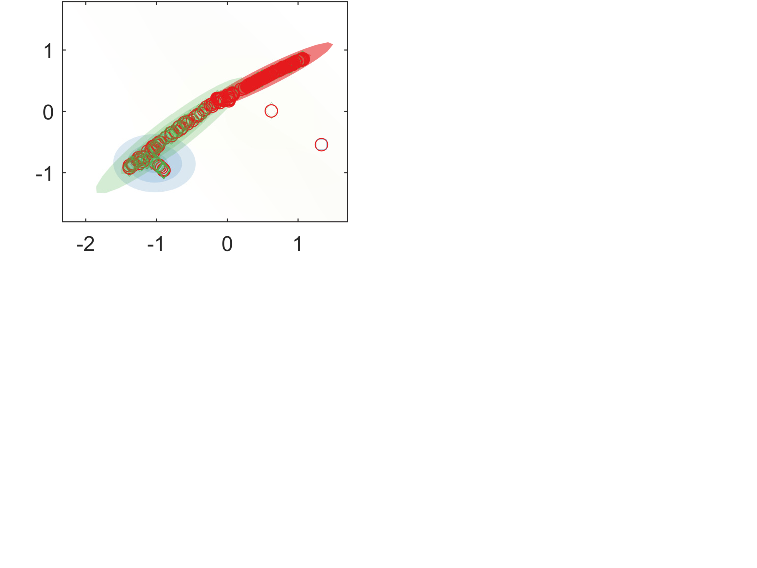
\includegraphics[width=0.45\linewidth]{img/lionlessMVMMexp3}
	\caption{Experimental results for the TOSCA dataset. Current mixture parameters, along with the latent positions for two shapes exhibiting different poses. Average Rand Index $0.6317$ }
\end{figure}
%\subsection*{Bayesian Multi-view Warped Mixture Model}
%
%Since we have a multi-view data set defined as $\mathcal{Y}=\left\{\mathbf{Y}^{v}\right\}_{v=1}^{V}$, where each view is set as $\mathbf{Y}^{v}\in \mathbb{R}^{N_v\times D_v}$, the joint likelihood is given by 
%
%
%\begin{align}
%p\left(\mathbf{Y},\mathbf{X},\mathbf{Z}\right) = \prod_{v=1}^{V}p\left(\setYv|\setFv,\setXv,
%\hParams\right)p\left(\setFv|\setXv\right)p\left(\setXv|\setZv\right)p\left(\setZv\right)
%\end{align}
%
%
%We assume that we have observations (inputs) in different views, in which observations are generated by mapping the latent coordinates through a set of smooth functions, over which Gaussian process priors are placed.
%
%\begin{align}
%p\left(\setYv|\setFv,\setXv,\setZv,\hParams\right) = \gD{\setYv|\setWv\setFv}{\beta^{-1}\eye}
%\end{align}
%


\bibliographystyle{plain}
\bibliography{bibRevTesisDoc}

\end{document}
